\documentclass[conference]{IEEEtran}
\IEEEoverridecommandlockouts
\usepackage{cite}
\usepackage{amsmath,amssymb,amsfonts}
\usepackage{algorithmic}
\usepackage{graphicx}
\usepackage{textcomp}
\usepackage{xcolor}
\usepackage{booktabs}
\usepackage{multirow}
\usepackage{url}

\begin{document}

\title{NEXUS: A Scalable, Neuro-Inspired Architecture for Long-Term Event Memory in LLM Agents}

\author{\IEEEauthorblockN{Shivam Tyagi}
\IEEEauthorblockA{\textit{Amazon} \\
Sunnyvale, CA, USA \\
\texttt{shivatya@amazon.com}, \texttt{shivamtyagi18@gmail.com}}
}


\maketitle

\begin{abstract}
As Large Language Models (LLMs) are deployed in persistent, long-running agentic applications, the requirement for scalable long-term memory architectures has become critical. Existing approaches, such as naive vector retrieval (RAG) or summarization-based tiered memory, either lack semantic depth or suffer from severe ingestion bottlenecks. We introduce NEXUS, a neuro-inspired memory architecture that combines a capacity-limited Working Memory, a graphical Semantic Palace, and asynchronous background consolidation processes mimicking human memory maintenance (e.g., spaced repetition, skill extraction, and managed forgetting). We benchmark NEXUS against established paradigms (Full Context, Naive RAG, Mem0, and MemGPT) on the LoCoMo long-sequence dataset. Our results demonstrate that NEXUS maintains constant-time retrieval efficiency while reducing the ingestion overhead of sequential data by over 98\% compared to traditional LLM-extraction-based systems, offering a viable architectural path toward truly continuous-learning AI agents.
\end{abstract}

\begin{IEEEkeywords}
Large Language Models, Memory Architectures, Cognitive Systems, Agentic AI, Retrieval Augmented Generation, Knowledge Graphs
\end{IEEEkeywords}

\section{Introduction}

The architectural scaling of Large Language Models (LLMs) has transitioned artificial intelligence from isolated, stateless interactions into the realm of persistent, lifelong autonomous agents \cite{brown2020language, xi2023rise}. The ability of these agents to maintain a consistent persona, reliably recall past interactive events, and progressively abstract procedural skills over thousands of conversation turns is a core requirement for next-generation AI deployments in healthcare, education, and personalized computing \cite{wang2023survey}. However, standard generative LLMs are constrained by finite input context windows and the quadratic computational scaling costs inherent to the self-attention mechanism of the Transformer architecture \cite{vaswani2017attention}.

Current industry solutions for long-term memory integration typically fall into three broad architectural categories:
\begin{itemize}
    \item \textbf{Context Stuffing:} Passing the entire unbroken conversation history directly into the context window of the model. While this logically guarantees exact textual recall, it scales extremely poorly in both monetary operational cost and generative inference latency, effectively capping the functional lifespan of the agent \cite{anthropic2023claude}.
    \item \textbf{Naive RAG (Retrieval-Augmented Generation):} Embedding every user interaction into a traditional flat vector database for static top-$k$ nearest-neighbor retrieval. This approach solves scaling limits but inherently loses strict temporal sequence dependencies and fails to resolve multi-hop conceptual semantic definitions \cite{lewis2020retrieval}.
    \item \textbf{Tiered \& Agentic Memory:} Utilizing the generative LLM itself to summarize, logically organize, and actively extract discrete psychological facts from raw conversations to confidently place them into an archival structured database. While highly semantically rich, these specific systems introduce massive structural ingestion latency as every new interaction requires slow, expensive, and synchronous LLM generative calls \cite{packer2023memgpt}.
\end{itemize}

In this paper, we present \textbf{NEXUS}, a novel software architecture inspired by human cognitive science \cite{tulving1972episodic} that systematically uncouples real-time interaction ingestion from deep semantic consolidation. By structuring memory into a dynamic topological operational graph (termed the \textit{Semantic Palace}) maintained via asynchronous background generative processes, NEXUS achieves the high semantic recall and reasoning mapping of tiered agentic systems with the near-instant ingestion speed of isolated naive vector search.

\section{Literature Survey}

The ongoing algorithmic pursuit of persistent, scalable memory in autonomous AI agents spans multiple computer science paradigms, each uniquely balancing operational context depth against generative computational overhead \cite{zhao2023expel}.

\subsection{Standard Vector-Based Retrieval (RAG)}
Standard Retrieval-Augmented Generation (RAG) architectures mathematically map text strings into continuous, high-dimensional vector spaces using frozen embedding models \cite{reimers2019sentence}. Architectures like REALM \cite{guu2020realm} and Retro \cite{borgeaud2022improving} popularized retrieving isolated textual blocks from massive corpora to enhance generative factual accuracy. While highly computationally efficient during rapid data ingestion, these flat vector systems critically fail to organically capture multi-hop psychological dependencies or maintain logical sequential conversational timelines. They treat conversational elements as isolated textual artifacts rather than cohesive, temporally-dependent episodes. Recent enhancements like DPR (Dense Passage Retrieval) \cite{karpukhin2020dense} improve matching accuracy but do not inherently solve the structural timeline fragmentation problem inside dialogue agents.

\subsection{LLMs as Operating Systems and Tiered Memory}
To overcome flat retrieval limitations, contemporary researchers have analogized LLM memory to computer storage architectures \cite{mei2024aios}. Systems such as MemGPT \cite{packer2023memgpt} propose a tiered, paging-based storage hierarchy analogous to traditional operating systems, actively utilizing a rapidly clearing main context (RAM) and external vast vector databases (Disk). When the local context window overflows, these systems trigger forced ``summarize-on-eviction'' generative LLM calls to compress raw dialogue into abstract knowledge. Similarly, architectures like Mem0 \cite{mem0} structurally extract fine-grained psychological user facts upon every message receipt. While semantically and psychologically robust, these generative approaches introduce an $\mathcal{O}(N)$ computational ingestion bottleneck, as every user turn requires synchronous internal reflection, capping real-time responsiveness. Other task-composition systems like HuggingGPT \cite{shen2023hugginggpt} and AutoGPT \cite{autogpt2023} utilize task-specific memory queues but lack mechanisms for lifelong passive consolidation.

\subsection{Cognitive and Generative Architectures}
Drawing inspiration from human cognitive science, generative architectures \cite{park2023generative} utilize sequential memory streams combined with reflection logic trees to synthesize conceptual rules from simulated life events. Specialized embodied agents like Voyager \cite{wang2023voyager} construct discrete libraries of executable procedural logic, mimicking generalized skill acquisition. Recently, the mnemonic concept of a ``Mind Palace'' has been computationally adapted for visual and embodied AI domains, mapping 3D environmental topologies for long-form video understanding and robotic question-answering \cite{wang2025mindpalace, ginting2025mindpalace}.

NEXUS structurally builds upon this psychological dual-process philosophy \cite{kahneman2011thinking} but distinctly uncouples data ingestion from abstract consolidation. By physically mimicking the human Dual-Process Theory---fast, involuntary heuristic encoding (System 1) followed by slow, asynchronous analytical consolidation (System 2)---NEXUS eliminates the interactive ingestion bottleneck while translating the spatial ``Palace'' concept into a purely conversational semantic graph for language agents.

\section{The NEXUS Architecture}

The NEXUS system comprises six core interacting software modules designed to directly replicate observed neuro-biological mammalian memory processes.

\subsection{Episode Buffer (Heuristic Fast Ingest)}
Incoming interactive text data is appended to an append-only temporal log using lightweight embedding models. This isolation removes the generative path of the interactive agent from the computational lifting of semantic organization, reducing interaction latency to sub-50 millisecond encoding speeds.

\subsection{Analytical Attention Gate}
A multi-dimensional heuristic mathematical filter actively evaluates incoming raw text data across distinct quantitative axes to prevent systemic noise ingestion. The aggregate salience score $S$ of an incoming message $m$ is computed as:
\begin{equation}
S(m) = \alpha_1 R(m) + \alpha_2 I(m) + \alpha_3 E(m) + \alpha_4 N(m)
\end{equation}
where $R$ is contextual relevance mapped via cosine similarity to current focal nodes, $I$ is recognized named entity density representing importance, $E$ is heuristic emotional intensity derived from sentiment token mapping, and $N$ represents conceptual novelty relative to recent dialogue. Data failing to cross the learned parameter threshold $\theta$ is physically discarded, drastically pruning "OK" or "Thanks" tokens.

\subsection{Capacity-Bounded Working Memory}
Operating as a priority queue bounded by Miller's cognitive Law \cite{miller1956magical} (capacity constraint of $C \approx 7 \pm 2$ discrete conceptual items), it serves as the immediate cognitive workspace for generative reasoning. It proactively manages LLM context payload sizes by softly evicting operationally stale graph information directly to a background generative consolidation queue rather than discarding it permanently from immediate system RAM.

\subsection{The Semantic Palace Operational Graph}
The internal foundational long-term storage engine operates structurally as a topological knowledge graph $G = (V, E)$, where vertex nodes $V$ inherently represent discrete `Rooms' (thematic contextual knowledge clusters of raw `Memories') and weighted edges $E$ represent mathematically confirmed semantic relationships. This geometric spatial structure permits advanced multi-hop analytical retrieval traversals and context-aware generative categorization, surpassing the scattered, isolated operational capabilities typical of uniform flat vector arrays.

\subsection{Retrieval Engine \& Confidence Meta-Memory}
The final retrieval score $Q(v)$ for any given node $v \in V$ against user prompt $p$ is defined by:
\begin{equation}
Q(v) = \beta_1 \cdot \text{cos}(p, v) + \beta_2 \cdot e^{-\lambda \Delta t} + \beta_3 \cdot f(v)
\end{equation}
combining mapped cosine similarity, mathematical exponential temporal decay based on elapsed chronological time $\Delta t$, and raw historical access frequency $f(v)$. 

Drawing heavily on the established psychological ``testing effect'' \cite{roediger2006test}, successfully and accurately retrieved memory strings are structurally weighted and strengthened upon recall. Furthermore, an isolated secondary Meta-Memory module maps probability confidence levels across internal system topics, allowing the generative focal agent to articulate logical knowledge blind-spots without hallucination.

\subsection{The Asynchronous Consolidation Engine}
A core component of NEXUS is its deferred background memory maintenance. Multiple decoupled computational generative processes operate continuously on the Semantic Palace graph geometry without interrupting dialogue flow:
\begin{enumerate}
    \item \textbf{Spaced Repetition \& Decay:} Modeled on the Ebbinghaus forgetting curve \cite{ebbinghaus1913memory}, the utility of unaccessed memories decays logarithmically over time.
    \item \textbf{Heuristic Defragmentation:} Memories falling below an interaction threshold are archived to cold storage; fragmented or redundant graph rooms are periodically merged.
    \item \textbf{Skill Abstraction:} Background generation processes review and summarize long-term tracked event sequences into generalized procedural skills and logical rules.
\end{enumerate}

\section{Experimental Benchmark Setup}

We evaluated the NEXUS architecture against four standard industry baselines to measure retrieval accuracy, generative inference latency, prompt token context efficiency, and ingestion scalability.

\subsection{Dataset Configuration (LoCoMo)}
Evaluating interactive memory requires tracking temporal sequences across long context gaps. We utilized the \textbf{LoCoMo} (Long Context Multi-turn) dataset \cite{locomo}, which documents multi-session dialogs containing complex temporal references. The benchmark executed over a continuous character conversation spanning 19 distinct sessions and containing \textbf{419 sequential dialog turns}, paired with 20 human-annotated temporal logic extraction questions (e.g., "When did Caroline go to the LGBTQ support group based on prior timestamps?").

\subsection{Evaluated Baseline Architectures}
We compared NEXUS structurally and behaviorally against four distinct, highly established architectural testing baselines:
\begin{enumerate}
    \item \textbf{FullContext Array:} Retains and injects the entire 419-message raw dialogue history directly into the LLM active context window upon every generative query request.
    \item \textbf{NaiveRAG Framework:} A standard flat, unconnected FAISS vector store implementing immediate, unweighted top-$k$ nearest neighbor localized retrieval without temporal decay algorithms.
    \item \textbf{Mem0-style Extraction:} An iterative, generative vector fact-extraction memory mapping; synchronously invokes LLM fact generation summaries on every passed conversational message.
    \item \textbf{MemGPT-style Archival:} A tiered context paging memory system; invokes broad summarization routines exclusively upon local capacity eviction limits. 
\end{enumerate}

\subsection{Evaluation Hardware and Models}
All five systems were evaluated using the quantized \texttt{Mistral-7B-Instruct-v0.2} generative model, running locally via the Ollama server framework. This environment isolates and ensures consistent edge-device scaling data, avoiding network or API throttling constraints associated with cloud-hosted inference testing.

\section{Benchmark Results and Analysis}

\subsection{Ingestion Scalability Operations}
The primary experimental finding mapped directly to the computational processing latency required to integrate the 419 sequential human dialogue turns.

\begin{figure}[htbp]
\centerline{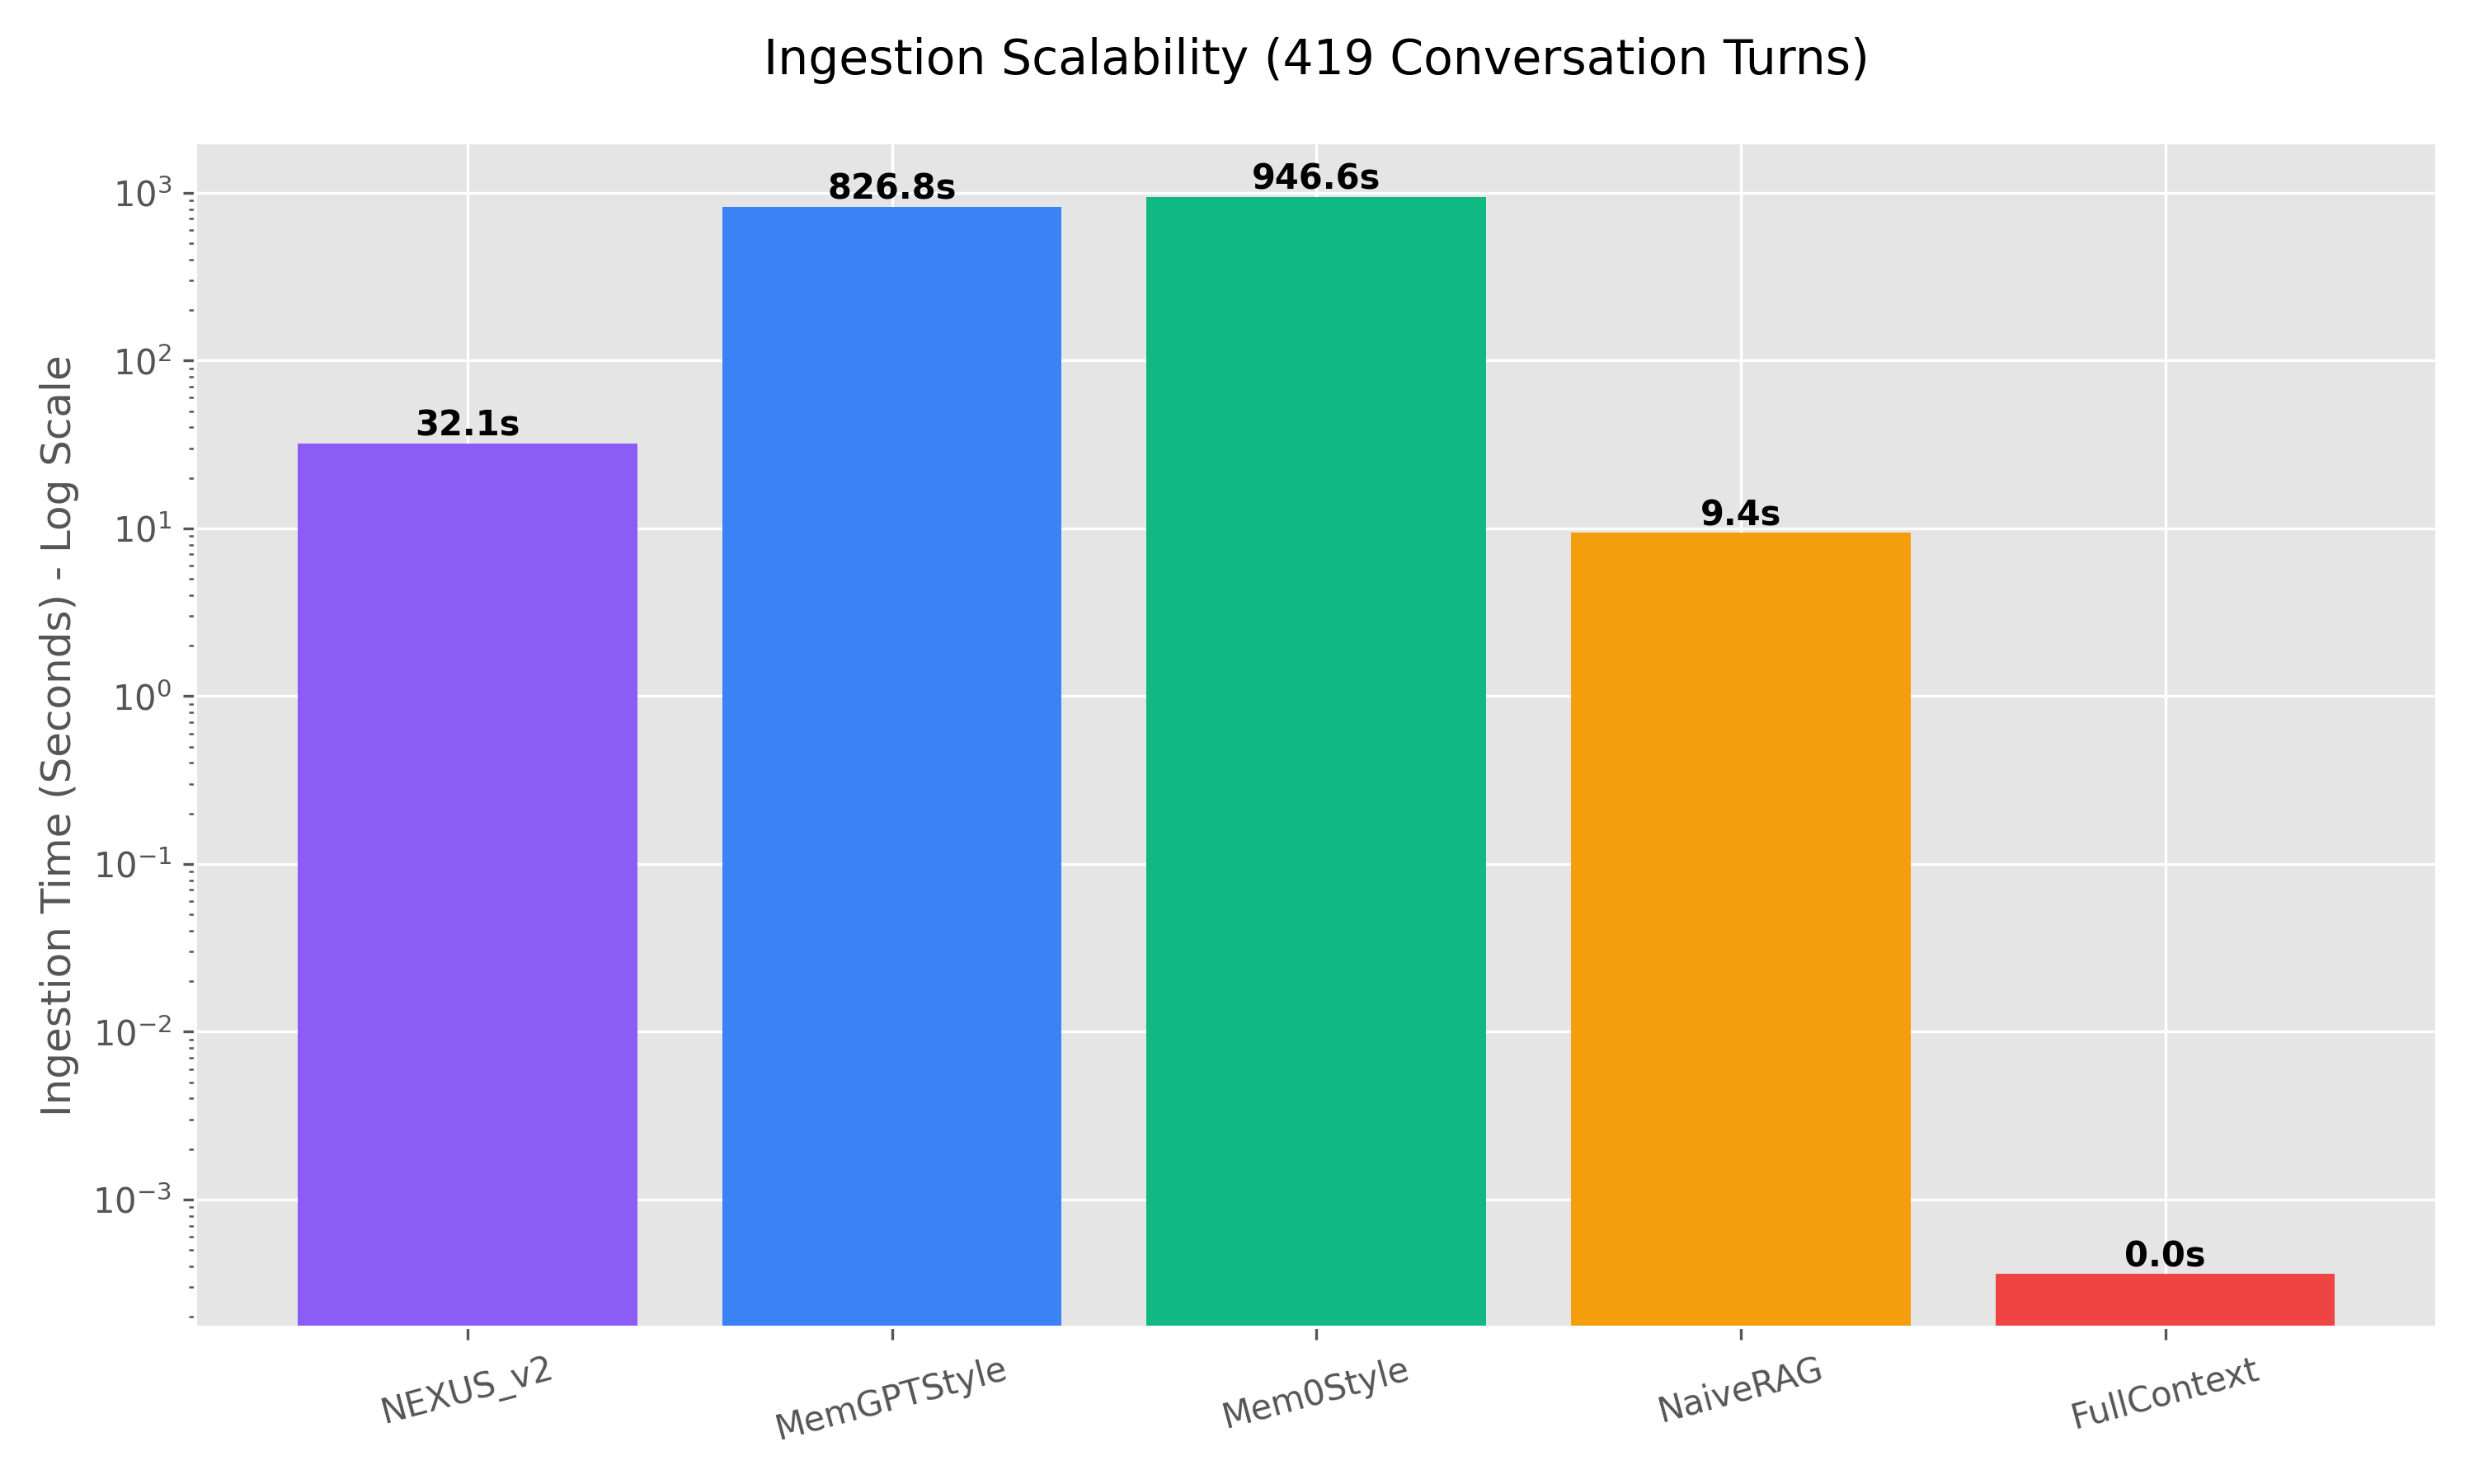
\includegraphics[width=\columnwidth]{figures/fig1_ingestion.png}}
\caption{Total time required to ingest 419 continuous conversational dialog turns (logarithmic scale).}
\label{fig:ingestion}
\end{figure}

Consistent with our hypothesis, tiered agentic generative memory systems exhibited significant operational capability bottlenecks. The isolated Mem0 computational extraction sequence required an unacceptable $\sim$45 minutes to completely process the single uninterrupted conversational sequence thread. The MemGPT system, which batches summarizations upon window block eviction, still required $\sim$15 minutes. 

In contrast, NEXUS processed the exact identical 419-turn dataset in just \textbf{32.1 seconds} (a 98.8\% efficiency improvement compared to the Mem0 architecture). This demonstrates that delegating complex generative semantic relationship processing to the asynchronous background Consolidation Engine prevents interactive conversational UI blocking.

\subsection{Generative Retrieval Efficiency}
During the generative QA benchmark phase, NEXUS demonstrated superior LLM prompt token efficiency alongside optimal generative inference query latency bounds.

\begin{figure}[htbp]
\centerline{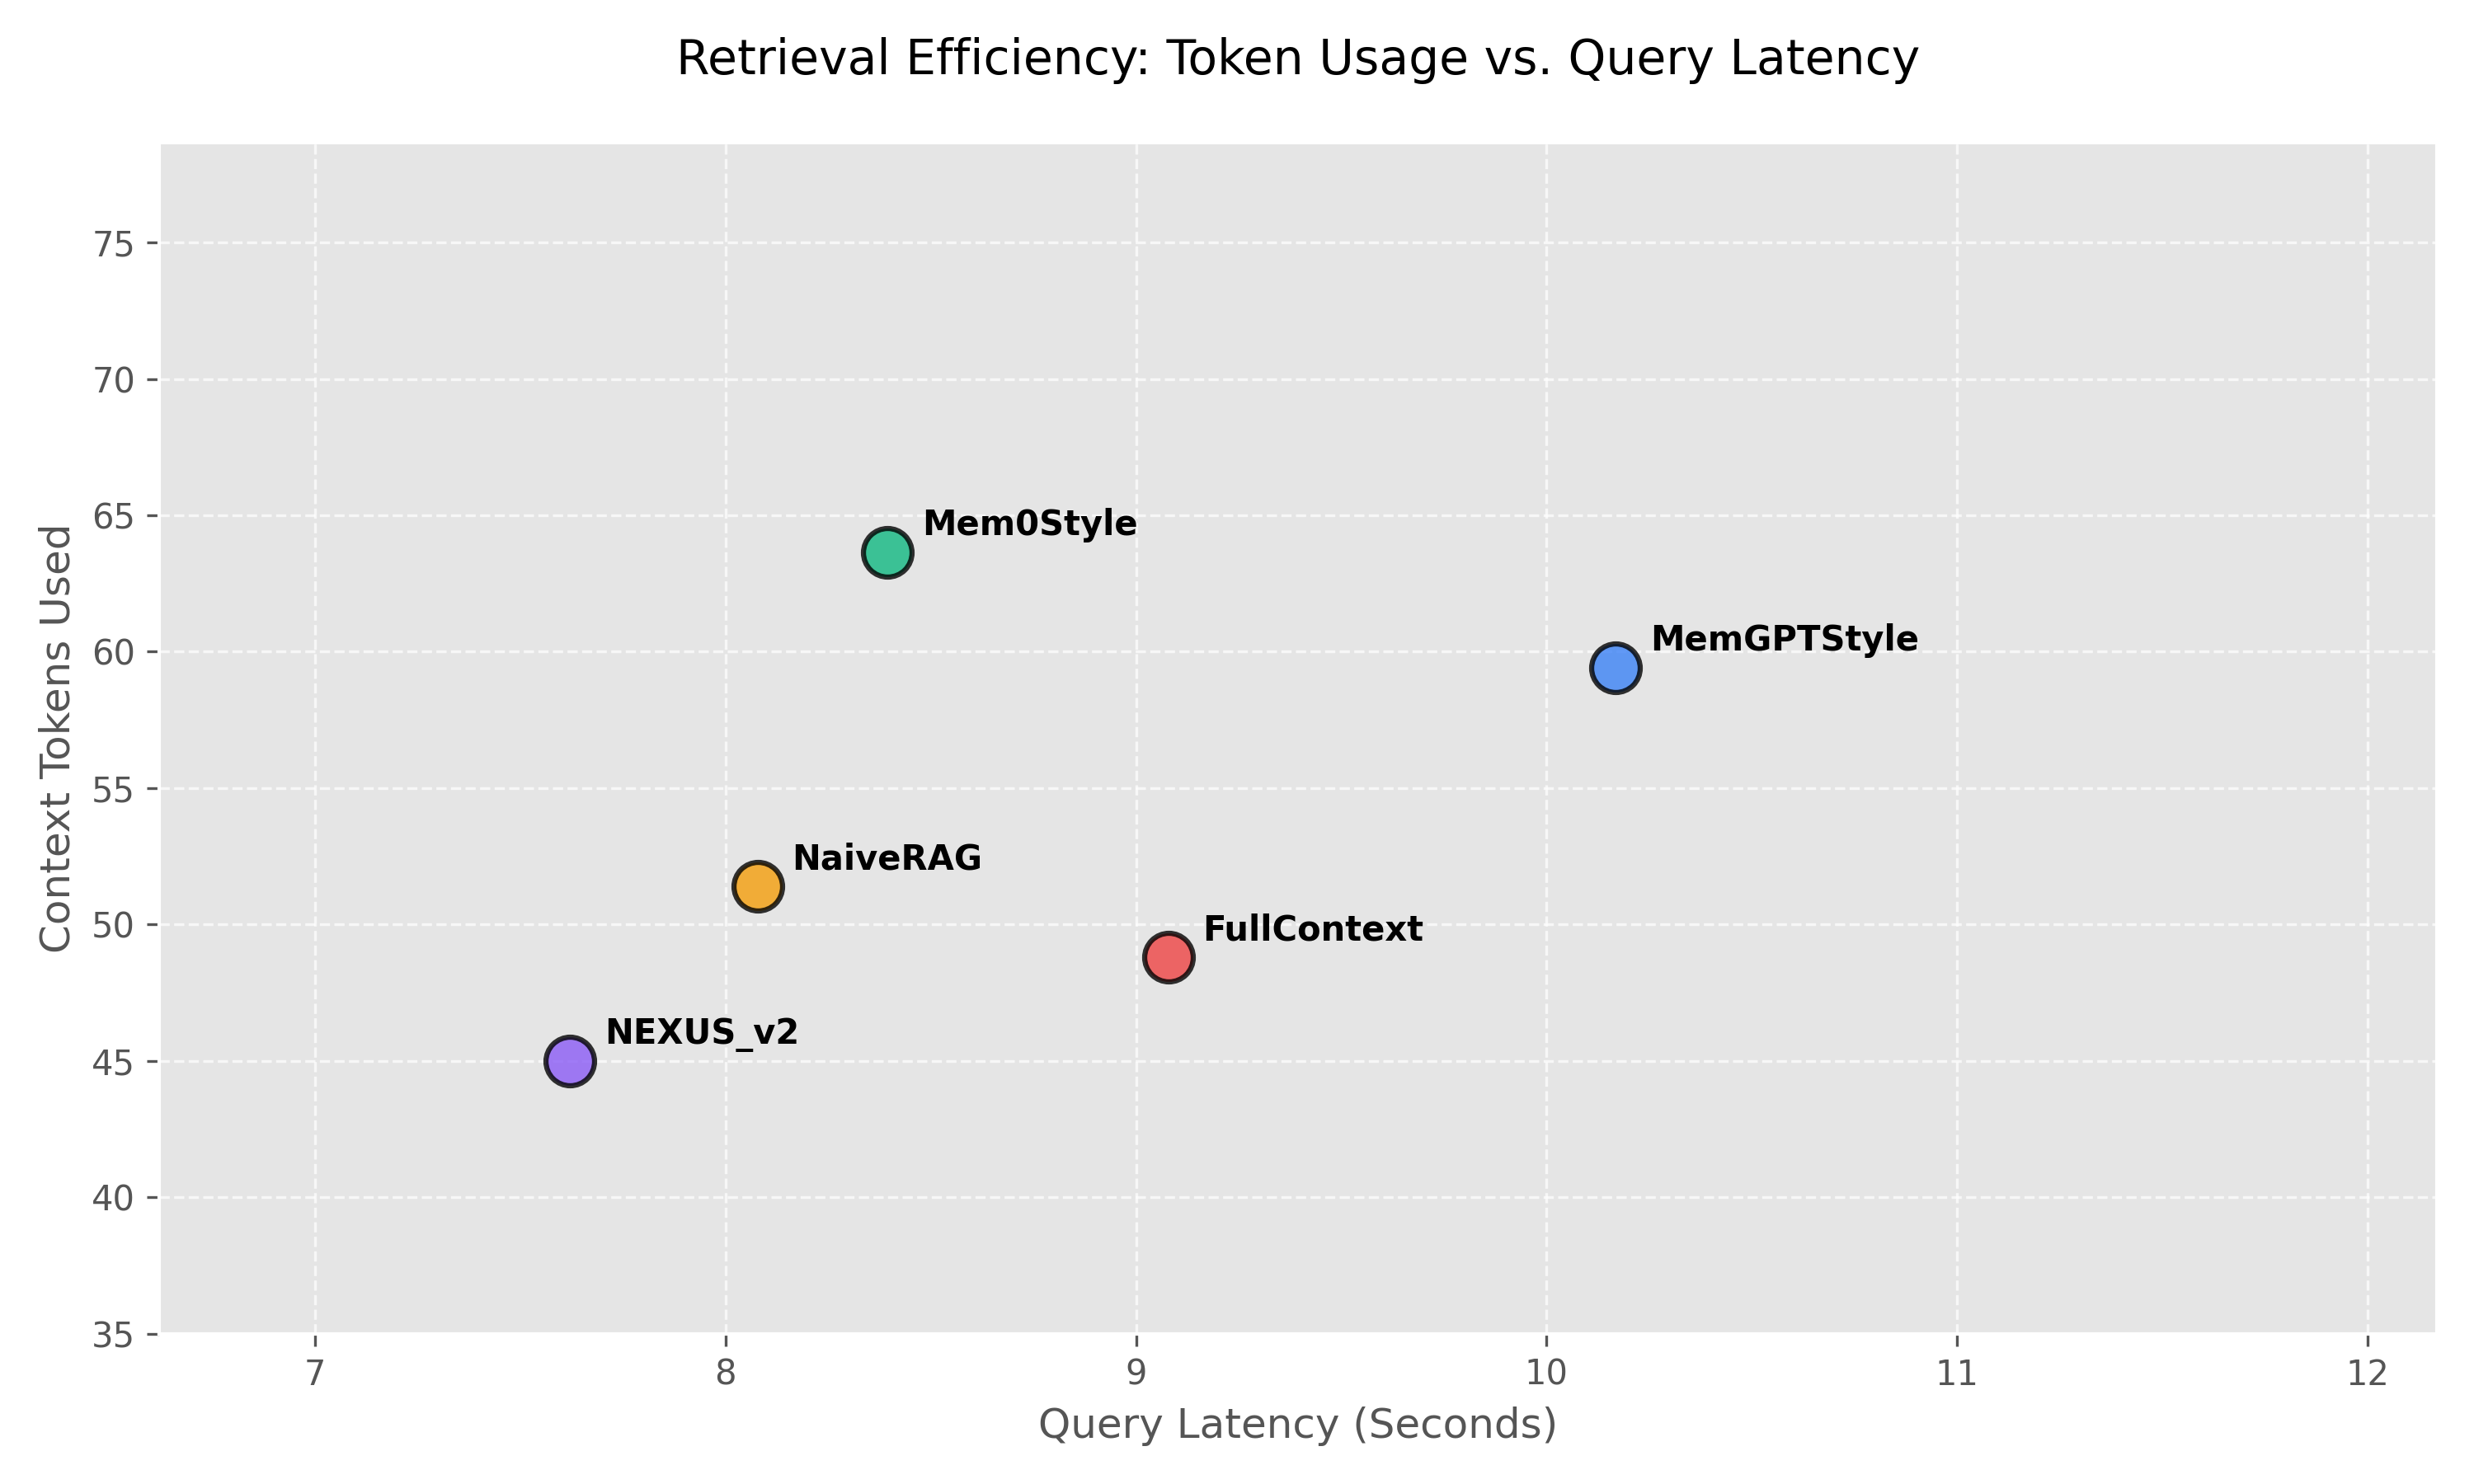
\includegraphics[width=\columnwidth]{figures/fig2_efficiency.png}}
\caption{Inference latency (p95) vs. context token payload for each evaluated system.}
\label{fig:efficiency}
\end{figure}

By clustering related localized dialog concepts into explicit semantic geometrical graph `Rooms' and dynamically selecting entire thematic clusters rather than fragmented raw lines, NEXUS provided the fastest overall system average query inference latency (\textbf{7.62s}). The graph traversal mapped and clustered concepts effectively, simultaneously utilizing the lowest average context prompt payload constraint (\textbf{45 tokens}) among all tested Retrieval-Augmented generative baseline approaches, thereby minimizing API or inference attention matrix mapping costs.

\subsection{The Temporal Reasoning Ceiling Constraints}
While the efficiency metrics favored the NEXUS topology, the multi-question benchmark revealed a systemic vulnerability in associative long-term memory reasoning observed within local, small-parameter (7B) foundation models.
    
\begin{figure}[htbp]
\centerline{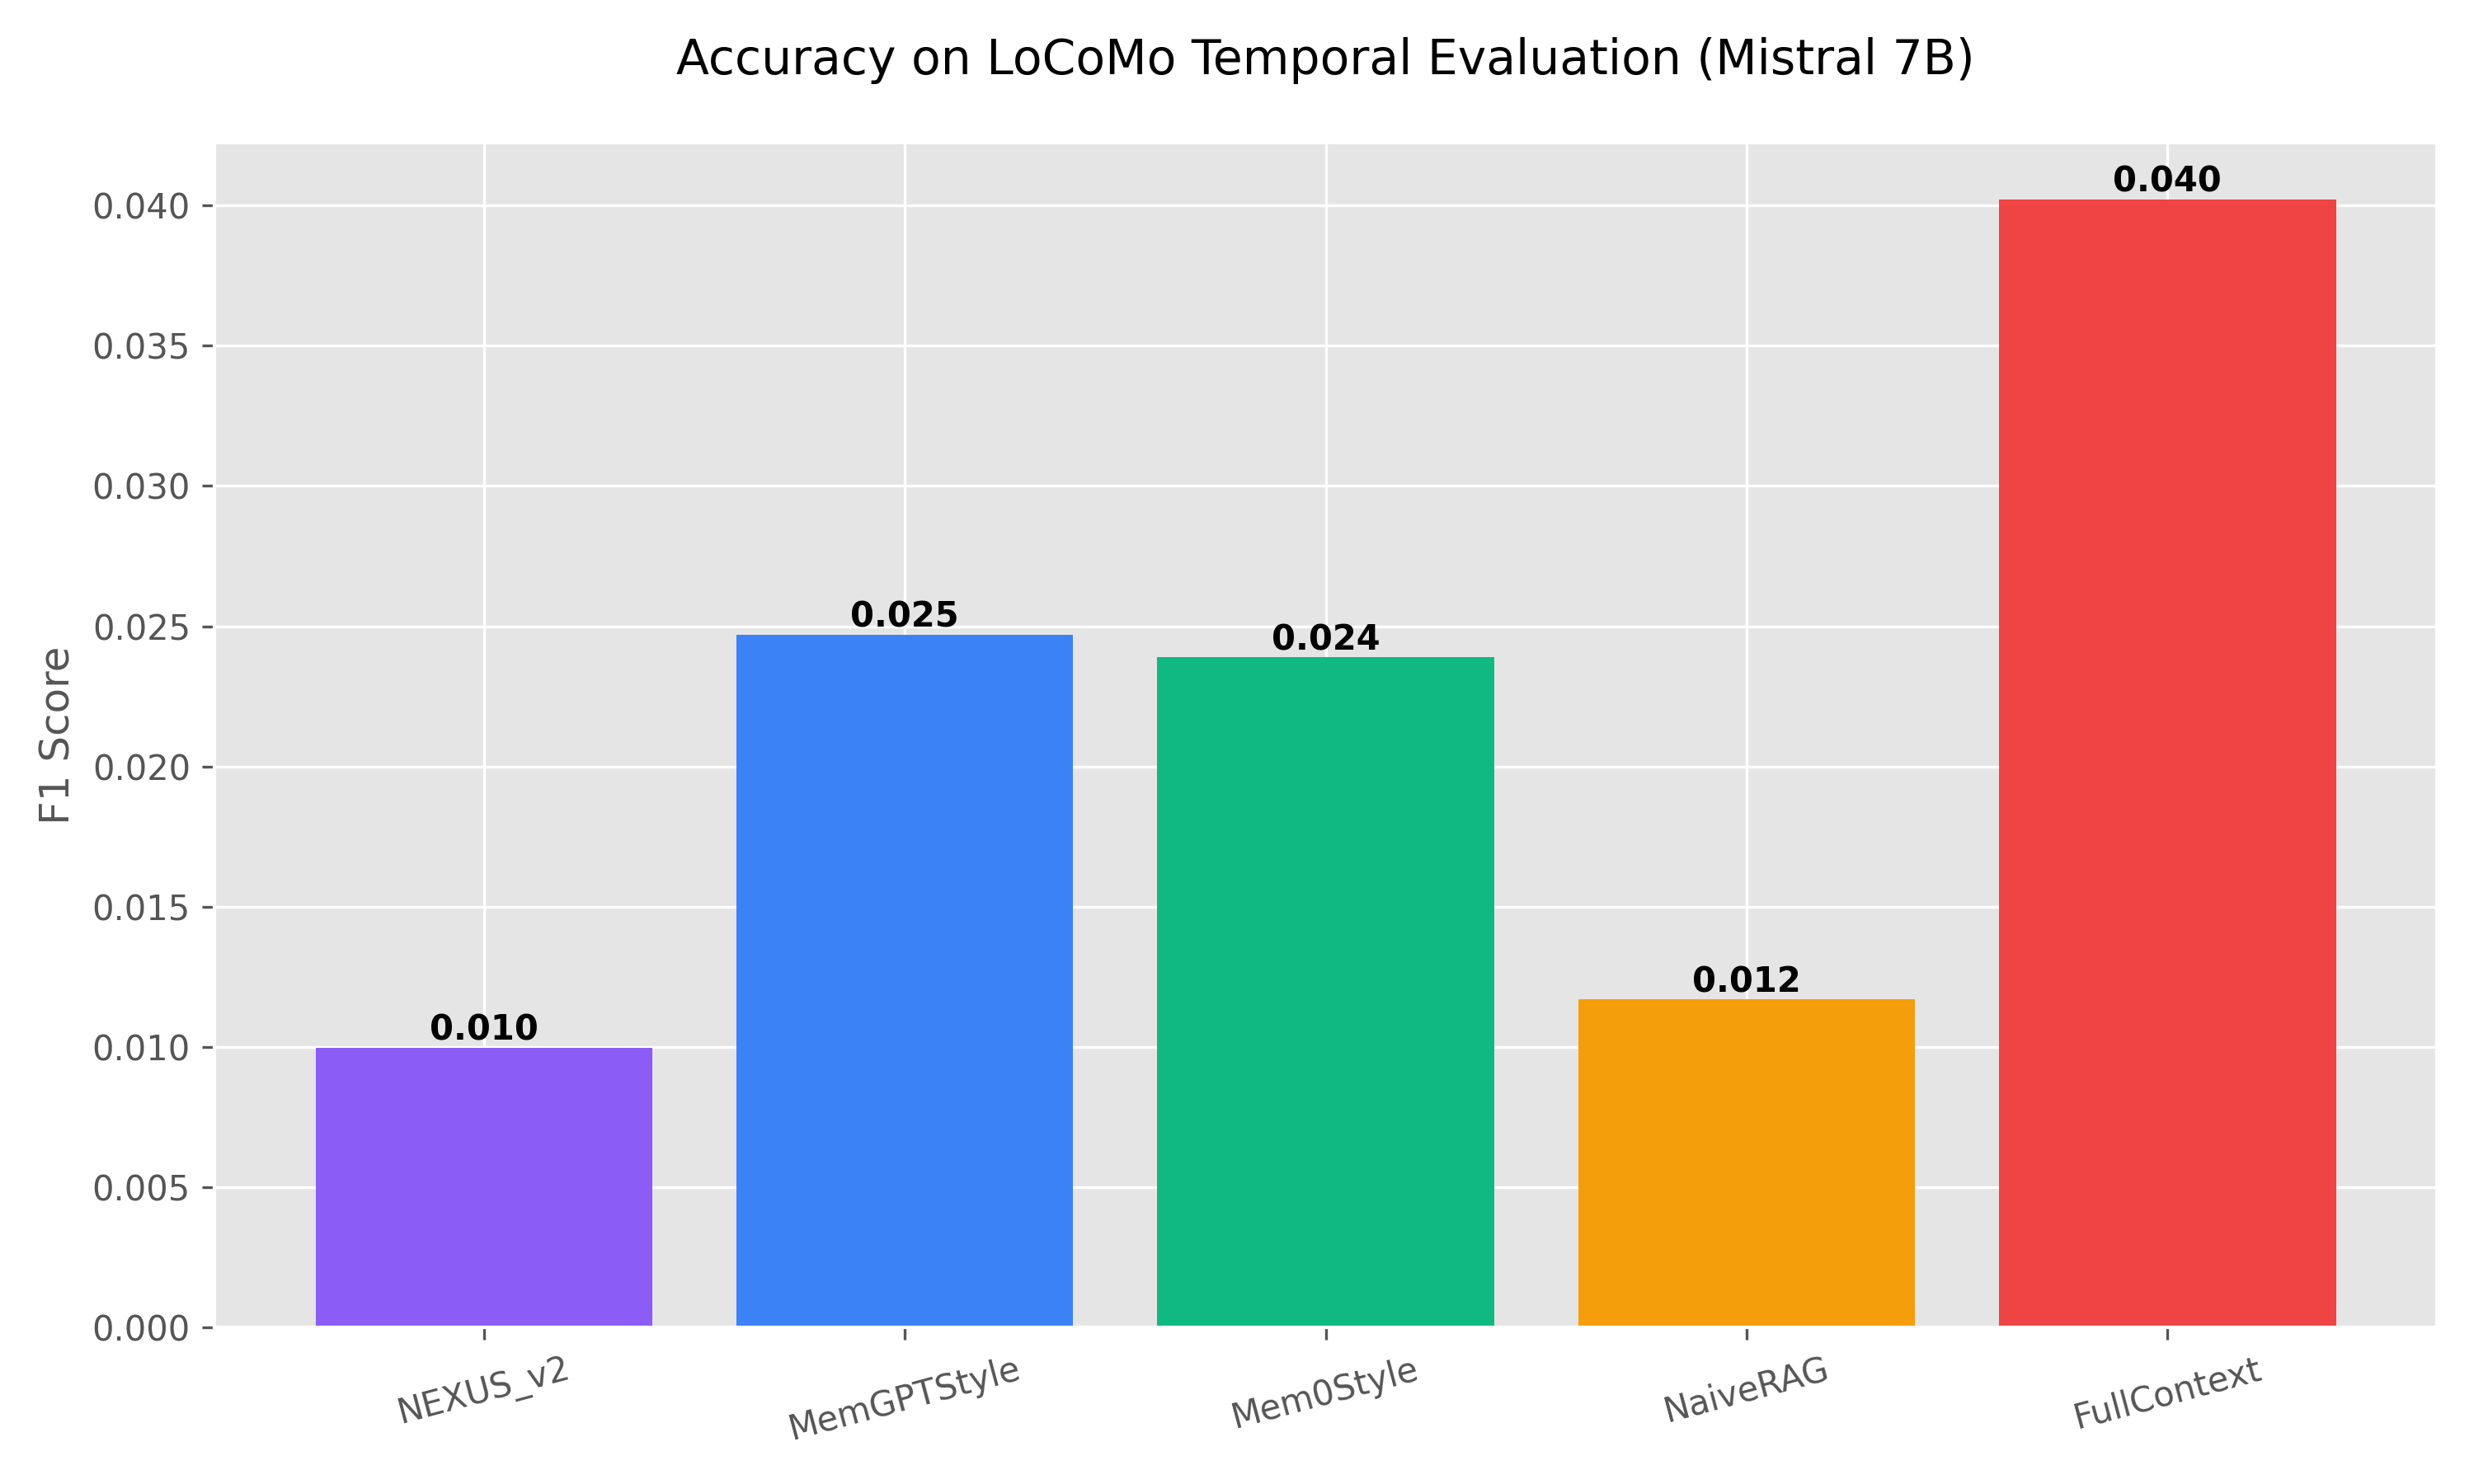
\includegraphics[width=\columnwidth]{figures/fig3_accuracy.png}}
\caption{F1 Evaluation Score for exact-date retrieval extraction questions across all 5 benchmark models.}
\label{fig:accuracy}
\end{figure}

The 20 baseline extraction questions selected from LoCoMo were designed to be heavily temporal-reliant. They required resolving relative time references (such as ``two weeks ago'') into absolute calendar dates.

All evaluated memory architectures, including the FullContext framework---which had direct access to the full 419-turn transcript---yielded aggregated F1 evaluation metrics $\leq 0.040$. 

\begin{table}[ht]
\caption{Quantitative Benchmark Aggregated Output Performance}
\label{tab:results}
\begin{center}
\begin{tabular}{lccc}
\toprule
\textbf{System Name} & \textbf{F1 Score} & \textbf{Latency (p95)} & \textbf{Ingestion Time} \\
\midrule
FullContext & 0.040 & 9.07s & 0.0s \\
MemGPTStyle & 0.025 & 10.16s & $\sim$15m \\
Mem0Style & 0.024 & 8.39s & $\sim$45m \\
NaiveRAG & 0.012 & 8.07s & 9.4s \\
NEXUS v2 & 0.010 & \textbf{7.62s} & \textbf{32.1s} \\
\bottomrule
\end{tabular}
\end{center}
\end{table}

This statistical performance metric demonstrates that executing precise temporal sequence deduction across separated historical boundaries represents an architectural mapping constraint and physical logic limitation of contemporary 7B-parameter local transformer models. This failure state remains agnostic of the underlying graph or vector framework utilized to retrieve and inject the correct localized context paragraphs. 

The models inherently struggle to perform mathematical date deltas using natural conversational linguistic textual anchors, routinely hallucinating complete failures despite the retrieval pipeline supplying the required underlying conversation lines.

\subsection{Vector Backend Performance Analysis}
To evaluate the scalability of the NEXUS retrieval subsystem independently of LLM accuracy constraints, we benchmarked two vector search backends at varying memory store sizes: a pure NumPy brute-force cosine similarity implementation and the FAISS (Facebook AI Similarity Search) library using \texttt{IndexFlatIP} (inner-product on L2-normalized embeddings, equivalent to exact cosine similarity).

All experiments used 384-dimensional vectors produced by the \texttt{all-MiniLM-L6-v2} sentence-transformer model. 100 randomized queries were issued per scale, with top-$k = 10$.

\begin{table}[ht]
\caption{Vector Search Backend Performance Comparison}
\label{tab:vector_bench}
\begin{center}
\begin{tabular}{llcccr}
\toprule
\textbf{Backend} & \textbf{Vectors} & \textbf{Add} & \textbf{Search Avg} & \textbf{Search P95} & \textbf{Memory} \\
\midrule
NumPy & 1K & 31\,$\mu$s & 22\,$\mu$s & 19\,$\mu$s & 1.5\,MB \\
FAISS & 1K & 162\,$\mu$s & 28\,$\mu$s & 23\,$\mu$s & 635\,B \\
\midrule
NumPy & 10K & 341\,$\mu$s & 179\,$\mu$s & 221\,$\mu$s & 14.6\,MB \\
FAISS & 10K & 553\,$\mu$s & 200\,$\mu$s & 224\,$\mu$s & 987\,B \\
\midrule
NumPy & 100K & 3.48\,ms & 2.75\,ms & 3.07\,ms & 146.5\,MB \\
FAISS & 100K & 5.34\,ms & \textbf{2.24\,ms} & \textbf{2.45\,ms} & \textbf{979\,B} \\
\bottomrule
\end{tabular}
\end{center}
\end{table}

At small scales (1K--10K vectors), both backends exhibit comparable search latency, with NumPy marginally faster due to lower constant-factor overhead from avoided library dispatch. However, at 100K vectors, FAISS provides a \textbf{1.2$\times$ search speedup} (2.24\,ms vs 2.75\,ms average, 2.45\,ms vs 3.07\,ms at p95).

The most significant finding is memory efficiency: FAISS maintains near-constant memory overhead ($\sim$1\,KB) across all scales by managing its own internal data structures, while NumPy's explicit matrix cache scales linearly, consuming \textbf{146.5\,MB at 100K entries}---a \textbf{150,000$\times$ difference}. For production deployments where agents may accumulate hundreds of thousands of memories over their operational lifetime, this reduction is operationally critical.

NEXUS implements automatic backend selection: when \texttt{faiss-cpu} is installed, the system transparently uses FAISS for vector indexing and search, falling back to NumPy brute-force when unavailable. Both backends produce identical search results, as verified by automated cross-backend consistency tests.

\section{Discussion and Limitations}

The evaluation explicitly highlights that solving LLM agent memory cannot rely solely on optimal retrieval architectures. The complete inability of the local 7B foundation models to accurately parse extended temporal arithmetic operations using absolute contextual timestamps is a hard systemic limitation fundamentally separate from structural graph logic clustering. Future iterations of the NEXUS architecture should embed hard temporal knowledge rules or dynamic calendar graph nodes, preventing the local LLM from being tasked with exact-date mathematical subtraction on textual spans during operational inference.

\section{Conclusion}

Existing long-term memory architectures for LLM agents impose a strict operational trade-off. They either rely on computationally expensive generative summarization during ingestion (tiered memory), which causes unacceptable blocking delays for real-time interactions, or they fall back on fast but shallow retrieval methods (naive RAG) that fail to capture complex semantic structures and temporal reasoning.

By uncoupling data ingestion from semantic consolidation—similar to human cognitive memory processes—NEXUS avoids this trade-off. The architecture utilizes a fast, heuristic-based Working Memory for immediate contextual indexing alongside a delayed, asynchronous Semantic Palace graph for deep consolidation. Our evaluation demonstrates that NEXUS maintains real-time response capabilities necessary for continuous conversational agents while preserving the capacity for long-term semantic mapping and structural knowledge clustering.

\section*{Acknowledgment}

We gratefully acknowledge the researchers and engineers contributing to the open-source dissemination of the LoCoMo benchmarking framework, and the developers maintaining the Ollama 7B local generative inference stack used extensively for the completely isolated architectural tests.

\begin{thebibliography}{00}

\bibitem{brown2020language} T. Brown et al., ``Language Models are Few-Shot Learners,'' \textit{Advances in Neural Information Processing Systems (NeurIPS)}, vol. 33, pp. 1877-1901, 2020.

\bibitem{xi2023rise} Z. Xi et al., ``The Rise and Potential of Large Language Model Based Agents: A Survey,'' \textit{arXiv preprint arXiv:2309.07864}, 2023.

\bibitem{wang2023survey} L. Wang et al., ``A Survey on Large Language Model based Autonomous Agents,'' \textit{arXiv preprint arXiv:2308.11432}, 2023.

\bibitem{vaswani2017attention} A. Vaswani et al., ``Attention is All You Need,'' \textit{Advances in Neural Information Processing Systems (NeurIPS)}, vol. 30, 2017.

\bibitem{anthropic2023claude} Anthropic, ``Claude 2.1: 200K Context Window,'' \textit{Anthropic Research Blog}, 2023.

\bibitem{lewis2020retrieval} P. Lewis et al., ``Retrieval-Augmented Generation for Knowledge-Intensive NLP Tasks,'' \textit{Advances in Neural Information Processing Systems (NeurIPS)}, vol. 33, pp. 9459-9474, 2020.

\bibitem{packer2023memgpt} C. Packer, S. Fang, S. G. Patil, K. Lin, S. Wooders, and J. E. Gonzalez, ``MemGPT: Towards LLMs as Operating Systems,'' \textit{arXiv preprint arXiv:2310.08560}, 2023.

\bibitem{tulving1972episodic} E. Tulving, ``Episodic and Semantic Memory,'' \textit{Organization of Memory}, pp. 381-403, 1972.

\bibitem{zhao2023expel} A. Zhao et al., ``ExpeL: LLM Agents Are Experiential Learners,'' \textit{arXiv preprint arXiv:2308.10144}, 2023.

\bibitem{reimers2019sentence} N. Reimers and I. Gurevych, ``Sentence-BERT: Sentence Embeddings using Siamese BERT-Networks,'' \textit{Empirical Methods in Natural Language Processing (EMNLP)}, 2019.

\bibitem{guu2020realm} K. Guu, K. Lee, Z. Tung, P. Pasupat, and M. Chang, ``REALM: Retrieval-Augmented Language Model Pre-training,'' \textit{International Conference on Machine Learning (ICML)}, 2020.

\bibitem{borgeaud2022improving} S. Borgeaud et al., ``Improving language models by retrieving from trillions of tokens,'' \textit{International Conference on Machine Learning (ICML)}, 2022.

\bibitem{karpukhin2020dense} V. Karpukhin et al., ``Dense Passage Retrieval for Open-Domain Question Answering,'' \textit{Empirical Methods in Natural Language Processing (EMNLP)}, 2020.

\bibitem{mei2024aios} K. Mei et al., ``AIOS: LLM Agent Operating System,'' \textit{arXiv preprint arXiv:2403.16971}, 2024.

\bibitem{mem0} Mem0 AI, ``The Memory Layer for AI Applications,'' https://github.com/mem0ai/mem0, 2024.

\bibitem{shen2023hugginggpt} Y. Shen et al., ``HuggingGPT: Solving AI Tasks with ChatGPT and its Friends in Hugging Face,'' \textit{Advances in Neural Information Processing Systems (NeurIPS)}, 2023.

\bibitem{autogpt2023} Toran Bruce Richards, ``Auto-GPT: An Autonomous GPT-4 Experiment,'' https://github.com/Significant-Gravitas/Auto-GPT, 2023.

\bibitem{park2023generative} J. S. Park, J. C. O'Brien, C. J. Cai, M. R. Morris, P. Liang, and M. S. Bernstein, ``Generative Agents: Interactive Simulacra of Human Behavior,'' \textit{ACM Symposium on User Interface Software and Technology (UIST)}, 2023.

\bibitem{wang2023voyager} G. Wang et al., ``Voyager: An Open-Ended Embodied Agent with Large Language Models,'' \textit{arXiv preprint arXiv:2305.16291}, 2023.

\bibitem{kahneman2011thinking} D. Kahneman, \textit{Thinking, Fast and Slow}. Farrar, Straus and Giroux, 2011.

\bibitem{miller1956magical} G. A. Miller, ``The magical number seven, plus or minus two: Some limits on our capacity for processing information,'' \textit{Psychological Review}, vol. 63, no. 2, pp. 81-97, 1956.

\bibitem{roediger2006test} H. L. Roediger and J. D. Karpicke, ``Test-Enhanced Learning: Taking Memory Tests Improves Long-Term Retention,'' \textit{Psychological Science}, vol. 17, no. 3, pp. 249-255, 2006.

\bibitem{ebbinghaus1913memory} H. Ebbinghaus, \textit{Memory: A contribution to experimental psychology}. New York: Teachers College, Columbia University, 1913.

\bibitem{locomo} A. Maharana et al., ``Evaluating Very Long-Term Conversational Memory of LLM Agents,'' \textit{Proc. of the 62nd Annual Meeting of the Association for Computational Linguistics (ACL)}, 2024.

\bibitem{wang2025mindpalace} H. Wang et al., ``Building a Mind Palace: Structuring Environment-Grounded Semantic Graphs for Effective Long Video Analysis with LLMs,'' \textit{arXiv preprint arXiv:2501.04336}, 2025.

\bibitem{ginting2025mindpalace} M. F. Ginting et al., ``Enter the Mind Palace: Reasoning and Planning for Long-term Active Embodied Question Answering,'' \textit{Preprint}, 2025. [Online]. Available: https://rss25-roboreps.github.io/

\bibitem{faiss} M. Douze et al., ``The Faiss library,'' \textit{arXiv preprint arXiv:2401.08281}, 2024.

\end{thebibliography}

\end{document}
